% A tangent vector v at a point p on a path c in U.
% Source: book/tex/diffgeo/forms.tex (§ Zero- and one-forms).
\documentclass[border=2mm]{standalone}
\usepackage{tikz}\usetikzlibrary{arrows.meta}\usepackage{amssymb}
\begin{document}
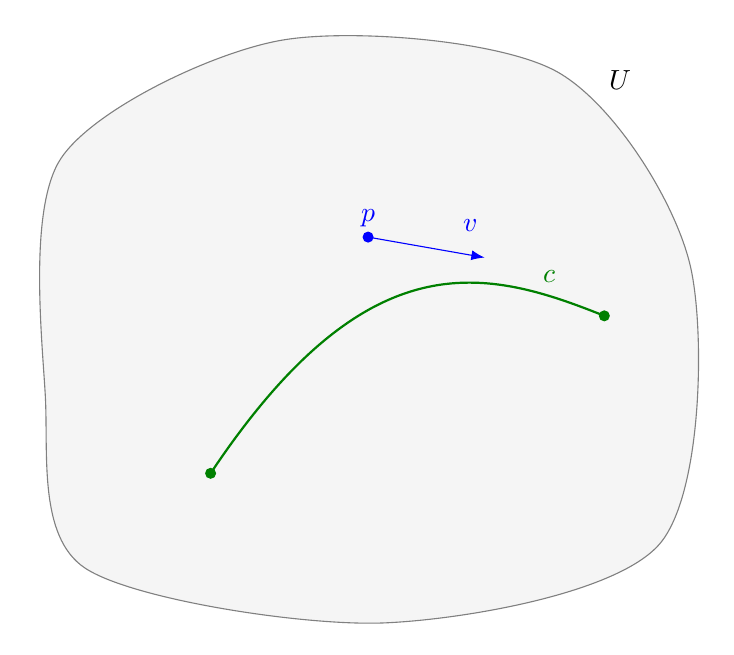
\begin{tikzpicture}
  \draw[gray,fill=gray!8] plot[smooth cycle] coordinates {(-3.6,-3.2)(0.2,-3.9)(3.7,-2.9)(4.1,0.6)(2.4,3.1)(-1.1,3.5)(-3.9,2)(-4.1,-1)}; \node at (3.2,3) {$U$};
  \draw[green!50!black,thick] (-2,-2) .. controls (0,1) and (1.5,0.6) .. (3,0);
  \fill[green!50!black] (-2,-2) circle (2pt);
  \fill[green!50!black] (3,0) circle (2pt);
  \node[green!50!black] at (2.3,0.5) {$c$};
  \fill[blue] (0,1) circle (2pt) node[above,blue]{$p$};
  \draw[blue,-{Latex}] (0,1)--(1.48,0.74);
  \node[blue] at (1.3,1.15) {$v$};
\end{tikzpicture}
\end{document}
